\section{Fixed-Kernel Identification and Information}
\label{app:proof}
The result in Proposition~\ref{prop:identification} holds for arbitrary normalized
nonnegative kernels under a fixed reference measure, including mixed measures.
It is conditional on their scientific grouping and on an interior weight.

If $p_w=p_{w'}$, then $v=w-w'\in\mathcal V_0$. Orthogonality of $\zeta$ therefore
makes $T_\zeta(w)=T_\zeta(w')$. Conversely, if $\zeta^\top v\ne0$ for some
$v\in\mathcal V_0$, every interior $w$ admits a sufficiently small nonzero
$t$ such that $w+tv$ stays in the simplex interior. Its density is unchanged,
but its target changes by $t\zeta^\top v$. This proves both directions.

For positive $w$, $f_j/p_w\le 1/w_j$ on the density support. Each score
component in (\ref{eq:information}) is therefore square integrable. For
$a\in\R^{K-1}$, $a^\top I_wa=0$ exactly when
$\sum_{j<K}a_j(f_j-f_K)=0$ almost everywhere. Its corresponding full null
direction is $(a_1,\ldots,a_{K-1},-\sum_{j<K}a_j)$. The target annihilates this
null space exactly when $\beta_\zeta$ belongs to the range of $I_w$.
When it does, $\phi_* =\beta_\zeta^\top I_w^+U$ is centered and satisfies
$\E_w(\phi_*U)=\beta_\zeta$. Any other centered square-integrable $\phi$ with
the same covariance has $\phi-\phi_*$ orthogonal to the score span. Hence
$\E_w(\phi^2)=\E_w(\phi_*^2)+\E_w\{(\phi-\phi_*)^2\}$, giving the bound.
This is an influence-function variance bound, not a claim that a particular
adaptive estimator attains it. Its sample-mean asymptotic variance factor is
conditional on fixed kernels; nuisance estimation is not covered.

\paragraph{Penalized uniqueness and likelihood identification.}
For $\tau>0$ and every $r_j>0$, consider
\[
 L_n(w)=\sum_i\log\{\textstyle\sum_jw_jf_j(x_i)\}
                   +\tau\sum_j r_j\log w_j.
\]
Assume all kernel values at observed points are finite, and each point has
positive density under some kernel. The prior
term forces the objective to minus infinity at the boundary; its Hessian adds
strictly positive curvature to the negative log likelihood. There is a unique
interior penalized maximizer, even for duplicate kernels. This optimization
fact does not alter the likelihood null space or establish branch-mass
identification. An empirical SVD can diagnose numerical rank for chosen
evaluation points, but it cannot prove population identification.

\section{Geometry, Coordinates, and a Temporal Extension}
\label{app:geometry}
\begin{proposition}[Coordinate transformation of branch targets]
\label{prop:coordinate-transport}
Let $\gamma_b:[0,1]\to\R^d$ be a one-to-one regular $C^1$ curve.
For an increasing $C^1$ diffeomorphism $s=\varphi(u)$, put
\[
 \widetilde\gamma_b(u)=\gamma_b\{\varphi(u)\},\qquad
 \widetilde h_b(u)=h_b\{\varphi(u)\}\varphi'(u),\qquad
 \widetilde K_b(\cdot\mid u)=K_b\{\cdot\mid\varphi(u)\}.
\]
Substitution in the branch integral leaves its probability law unchanged.
For an exact branch, the chain rule gives
\[
 \frac{\widetilde h_b(u)}{\|\dot{\widetilde\gamma}_b(u)\|}
 =\frac{h_b\{\varphi(u)\}}{\|\dot\gamma_b\{\varphi(u)\}\|},
\]
which is the same density per unit physical arc length. Normalized arc length
is
\[
 u_b(s)=\frac{\int_0^s\|\dot\gamma_b(v)\|\,dv}
                  {\int_0^1\|\dot\gamma_b(v)\|\,dv}.
\]
The distribution of $u_b(S)$ is invariant to the coordinate transport above
when branch origin and orientation agree. Shared branch correspondence is
still needed for a comparison across groups. In contrast, the transformed
coordinate mean is
$\int_0^1\varphi^{-1}(s)h_b(s)\,ds$ and need not equal the original mean.
\end{proposition}
\begin{proof}
Substitute $s=\varphi(u)$ in the branch integral and coordinate mean.
The chain rule gives
$\|\dot{\widetilde\gamma}_b(u)\|
=\|\dot\gamma_b\{\varphi(u)\}\|\varphi'(u)$, proving both the intrinsic
density and normalized arc-length identities.
\end{proof}
For a full-rank counterexample, take $\gamma(s)=(s,0)$, $h(s)=1$ and
$K(dx\mid s)=\Normal(dx;(s,0),\sigma^2I_2)$, with $\sigma>0$.
For $\kappa\ne0$, put
\[
 \varphi_\kappa(u)=\frac{e^{\kappa u}-1}{e^\kappa-1},\qquad
 \widetilde h_\kappa(u)=\frac{\kappa e^{\kappa u}}{e^\kappa-1},\qquad
 \widetilde\gamma_\kappa=\gamma\circ\varphi_\kappa.
\]
Every $\kappa$ gives the same observed law, but the transformed coordinate
mean is $e^\kappa/(e^\kappa-1)-1/\kappa$, with limit $1/2$ and derivative
$1/12$ at zero. Thus fixed endpoints and positive tube covariance alone do
not identify a coordinate mean. On a self-overlapping immersion,
the density relative to Hausdorff measure sums the Jacobian-adjusted
contributions over coordinate preimages; Equation~\ref{eq:intrinsic} uses
the one-to-one case.

\paragraph{Skeleton and observed support.}
A finite collection of curve edges and declared vertices can be organized
as a metric graph, allowing endpoints, junctions, and cycles. This describes
the latent representation. A positive-mass full-rank Gaussian component has
support throughout $\R^d$, so the topology of a noisy observed distribution
differs from the connectivity of its centerlines. The formulation here uses
declared structure and does not provide a topology-recovery theorem.

The tangent-normal covariance in Equation~\ref{eq:frame} is Euclidean.
The locally adaptive normal distribution (LAND) instead uses a learned
Riemannian metric, geodesic distance, and normalization relative to
Riemannian volume \citep{arvanitidis2016land}. To use such a distribution
as an SFD kernel, its law must be expressed relative to the same declared
reference measure as the other components.

\subsection{A Projected Fermat-Quintic Section}
\label{app:fermat-construction}
The Fermat quintic
$\mathcal Q=\{\sum_{j=0}^4z_j^5=0\}\subset\mathbb{CP}^4$
is a standard Calabi--Yau example \citep{hendi2024invariant}.
Fixing projective coordinates $[-1:z_1:z_2:0:0]$ selects the affine curve
$z_1^5+z_2^5=1$, of two real dimensions. For $w=u+iv$, put
\begin{equation}
 \begin{split}
 z_1&=e^{2\pi i k/5}(\sin w)^{2/5},\qquad
 z_2=e^{2\pi i \ell/5}(\cos w)^{2/5},\\
 F(u,v;k,\ell)&=\bigl(\operatorname{Re}z_1,\operatorname{Re}z_2,
              (\operatorname{Im}z_1+\operatorname{Im}z_2)/\sqrt2\bigr),
 \end{split}
 \label{eq:fermat-projection}
\end{equation}
where $k,\ell\in\{0,\ldots,4\}$ and the powers use the principal complex
logarithm. Since $\sin^2w+\cos^2w=1$, every generated pair satisfies the
section equation. Figure~\ref{fig:fermat-section} plots $F$ on
$u\in[0.025,\pi/2-0.025]$, $v\in[-1,1]$.

The observation law uses 13 equally spaced fixed values of $v$ for each of
the 25 root pairs. Each resulting curve has uniform $u$, mass $1/325$ and
Gaussian covariance $0.035^2I_3$. Thus an SFD with one-dimensional coordinate
domains supplies a finite-curve approximation to the projected patches.
Its full-rank observation law is defined in $\R^3$; its latent sampling rule
is a coordinate-grid mixture rather than Calabi--Yau volume. The example
concerns a projected section, not the full six-real-dimensional manifold or
its Ricci-flat metric.

In Figure~\ref{fig:fermat-section}, colors identify the first root index
$k$. The smooth patch display uses continuous $v$, while its observation
law uses the finite grid described above.

\FloatBarrier

\subsection{A Temporal Extension}
A possible temporal model would couple the observation kernels to a process
on an oriented metric graph. An edge occupancy density $\rho_b(s,t)$ could
satisfy
\[
 \partial_t\rho_b=-\partial_s j_b,\qquad
 j_b=v_b\rho_b-\partial_s(D_b\rho_b),\qquad D_b>0.
\]
Such a model also requires an initial law, probability-conserving vertex
conditions, and any vertex-mass dynamics. Graph diffusion has established
generator and vertex-boundary constructions \citep{kostrykin2012brownian}.
Estimating drift, diffusion, or passage times would require time-ordered
trajectories, sampling intervals, trajectory identifiers, and a treatment of
sampling bias. Static occupancy alone does not identify those quantities.
This is an extension of the observation model, not a fitted result in this paper.

\FloatBarrier

\section{Figure Construction and Additional Examples}
\label{app:visual-examples}
\subsection{Construction of the Main-Text Displays}
Figure~\ref{fig:elvis-example} uses 32 grayscale contours selected inside
an annotated foreground region, plus photo-guided paths for the outer pose,
microphone and cable. Curve weights are proportional to arclength, occupancy
is uniform in normalized arclength, and kernel covariance is $0.014^2I_2$.
The 18,000 draws use seed 2026102205. Its density display uses 4096 midpoint
nodes per curve, a $500\times500$ grid and Gaussian convolution. Coordinates
are scaled image-plane coordinates; photographic brightness does not set
component mass.

Figure~\ref{fig:volcano} uses the circular-tube law specified in the main
text, with 16,000 draws and seed 2026102206. Its $64\times64$ bivariate
histogram displays $[-2.25,2.25]^2$, containing 15,853 observations; the
remaining 147 draws are outside this window. Bin density divides by the
full sample size and bin area. All radii enter the lower histogram.
Figure~\ref{fig:fermat-section} uses 18,000 draws and seed 2026102207
from the finite-curve law in Appendix~\ref{app:fermat-construction}.

Figure~\ref{fig:reference-histograms} uses the first two coordinates of
a ten-dimensional correlated Gaussian, a ten-dimensional skew mixture and
a two-dimensional banana transform. All 500 stored training observations
from repetition~1 of each reference scenario enter the histograms. The
$24\times24$ joint bin densities use count divided by sample size and bin
area and integrate to one. The lower panels are first-coordinate marginals.

\subsection{Three-Dimensional and Other Specified Laws}
Figure~\ref{fig:face-example} shows a three-dimensional law, retaining its
third-coordinate observations. Its localized Gaussian components have
positive covariance, whereas an exact atom in Definition~\ref{def:sfd}
is a point mass. The main-text density surfaces in
Figure~\ref{fig:density-examples} use the first two coordinates instead.
Their displayed heights are proportional to $(p/\max p)^a$, with
panel-specific exponents $a=0.28,0.1664,0.36,0.36$ for the snowflake,
face, maze and ECG-like laws. Colors also use panel-specific nonlinear
relative scales. The face uses tube SD 0.070 and blob SD 0.105, different
from the narrower sample illustration below. These displays are specified
laws, without fitted-method comparisons.

\begin{figure}[t]
\centering
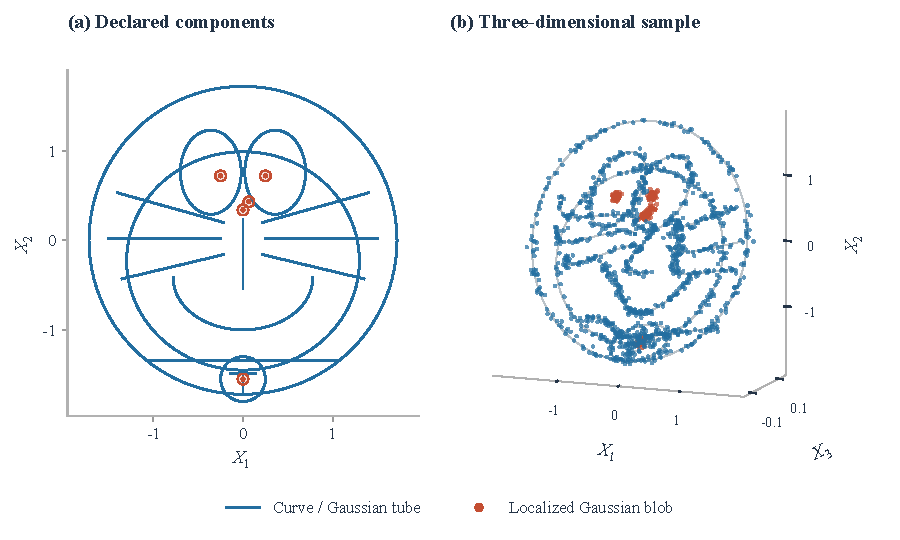
\includegraphics[width=0.93\linewidth,clip]{figures/face_example_3d.pdf}
\caption{A stylized-face SFD with 16 Gaussian tubes and five localized
Gaussian components. Left: projected centerlines and blob contours at
squared Mahalanobis distance four. Right: all 1,600 observations in three
dimensions, with gray centerlines as guides. Blue and red identify tubes
and blobs. Branch coordinates are uniform on $[0,1]$; SDs in the first two
coordinates are 0.020 for tubes and 0.030 for blobs, and the
third-coordinate SD is 0.012. The right panel uses actual $X_3$ values with
unequal display scales.}
\label{fig:face-example}
\end{figure}

\FloatBarrier


\section{Distributional Calculus}
\label{app:calculus}
All statements use the finite component sets and measurable kernels of
Definition~\ref{def:sfd}. Exact atoms are Dirac laws; regularized blobs can
be represented among the continuous residual components. Component labels
are latent and need not partition the observed space.

\begin{proposition}[Normalization and latent construction]
\label{prop:normalization}
The SFD law is the marginal of the following construction: draw a component
$Z$ with probabilities $\pi_c$; given an atom, set $X=\xi_a$; given a branch,
draw $S$ with density $h_b$ and then $X\sim K_b(\cdot\mid S)$; given a
residual, draw $X$ with density $q_r$. In particular, $P_\theta(\mathcal X)=1$.
\end{proposition}
\begin{proof}
Each branch integral is a measure: for disjoint measurable sets,
monotone convergence passes their sum through the nonnegative kernel
integral. It has total mass $\int h_b(s)K_b(\mathcal X\mid s)\,ds=1$.
The finite nonnegative mixture therefore has total mass $\sum_c\pi_c=1$.
Conditioning the stated latent construction on $Z$ gives exactly its
probability on every measurable set, proving equality of laws.
\end{proof}

\begin{proposition}[Mixed-density evaluation]
\label{prop:mixed-density}
For fixed atom locations and fixed exact branch maps, a common reference is
\[
 \nu=\lambda_d+\sum_a\delta_{\xi_a}
            +\sum_{b\in\mathcal B_{\mathrm{ex}}}(\gamma_b)_\#ds,
\]
where $ds$ is restricted to the finite-volume coordinate domain. If $P_c$
denotes each normalized component law, then
\[
 p_\theta=\sum_c\pi_c\frac{dP_c}{d\nu}.
\]
For a continuous component with Lebesgue density $g_c$, its common-reference
density is $g_c\rho$, where $\rho=d\lambda_d/d\nu$. For an injective exact
branch, put $\nu_{\Gamma,b}=(\gamma_b)_\#ds$. Its contribution is
\[
 \pi_b h_b\{\gamma_b^{-1}(x)\}
                    \frac{d\nu_{\Gamma,b}}{d\nu}(x).
\]
Thus overlapping reference contributions must be converted before addition.
\end{proposition}
\begin{proof}
The branch reference measures are finite and their finite sum with Lebesgue
measure is sigma-finite. A coordinate null set has zero probability under
$h_b(s)ds$, so its pushforward probability is dominated by its pushforward
reference. All components are therefore dominated by $\nu$. Linearity of
the Radon--Nikodym derivative gives the mixture formula; its chain rule gives
the continuous and injective-branch expressions. In particular, a continuous
density contributes zero mass at an exact atom, even if its Lebesgue density
there is positive.
\end{proof}

For a regular immersion of intrinsic dimension $m_b$ with finite preimages,
the area formula gives, at almost every point of its image,
\[
 \frac{dP_b}{d\mathcal H^{m_b}}(x)
   =\sum_{s:\gamma_b(s)=x}\frac{h_b(s)}{J_b(s)},\qquad
 J_b(s)=\sqrt{\det\{D\gamma_b(s)^\top D\gamma_b(s)\}}>0.
\]
Relative to the branch's own pushforward reference, the density is the ratio
of this sum to $\sum_{s:\gamma_b(s)=x}1/J_b(s)$, not the unweighted sum of
coordinate densities. The common-reference conversion still applies.

\subsection{Expectation, Moments and Covariance}
For completeness, Proposition~\ref{prop:expectation} follows first for
nonnegative $g$ by conditioning on $Z$, then $S$, and using Tonelli's theorem.
For integrable signed $g$, apply the same argument to $g^+$ and $g^-$ and
subtract. This proves the full identity without a Lebesgue-only assumption.

In the Gaussian-tube case, whenever the second moments exist,
\begin{align*}
 \mu=\E_\theta X
 &=\sum_a\pi_a\xi_a+\sum_b\pi_b\int h_b(s)\gamma_b(s)\,ds
                         +\sum_r\pi_r\E_{q_r}X,\\
 \E_\theta(XX^\top)
 &=\sum_a\pi_a\xi_a\xi_a^\top
   +\sum_b\pi_b\int h_b(s)
       \{\gamma_b(s)\gamma_b(s)^\top+\Sigma_b(s)\}\,ds
   +\sum_r\pi_r\E_{q_r}(XX^\top).
\end{align*}
The covariance is $\E_\theta(XX^\top)-\mu\mu^\top$. A branch covariance
therefore separates variation of $\gamma_b(S)$ from the average conditional
noise covariance $\int h_b(s)\Sigma_b(s)\,ds$. If the component moment
generating functions and the following integrals are finite near the origin,
\[
 M_X(t)=\sum_a\pi_a e^{t^\top\xi_a}
 +\sum_b\pi_b\int h_b(s)
   e^{t^\top\gamma_b(s)+t^\top\Sigma_b(s)t/2}\,ds
 +\sum_r\pi_r M_{q_r}(t).
\]
Both formulas are choices of $g$ in the master identity.

\subsection{Marginal and Conditional Laws}
Let $J$ be a nonempty proper subset of coordinate indices, put $Y=X_{-J}$,
and write $T_J$ for projection onto $X_J$.

\begin{proposition}[Marginal law]
\label{prop:marginal}
For arbitrary SFD kernels,
\[
 (T_J)_\#P_\theta
  =\sum_a\pi_a\delta_{\xi_{a,J}}
    +\sum_b\pi_b\int h_b(s)(T_J)_\#K_b(\cdot\mid s)\,ds
    +\sum_r\pi_r(T_J)_\#Q_r.
\]
For Gaussian tubes, the projected branch kernel is
$\Normal(\gamma_{b,J}(s),\Sigma_{b,JJ}(s))$. Exact branches instead use
their projected pushforward laws, which may change dimension or acquire atoms.
\end{proposition}
\begin{proof}
Evaluate the original law on $T_J^{-1}(A)$ for a measurable set $A$.
Projection commutes with the finite sum and nonnegative kernel integral.
The Gaussian assertion is the marginal formula for a multivariate normal.
\end{proof}

\begin{proposition}[Gaussian branch conditional law]
\label{prop:gaussian-conditional}
For a full-rank Gaussian branch kernel, conditional on $(Z=b,S=s,Y=y)$,
$X_J$ is Gaussian with mean and covariance
\begin{align*}
 m_{J\mid-J,b}(s;y)
 &=\gamma_{b,J}(s)+\Sigma_{b,J,-J}(s)\Sigma_{b,-J,-J}(s)^{-1}
                         \{y-\gamma_{b,-J}(s)\},\\
 V_{J\mid-J,b}(s)
 &=\Sigma_{b,JJ}(s)-\Sigma_{b,J,-J}(s)
            \Sigma_{b,-J,-J}(s)^{-1}\Sigma_{b,-J,J}(s).
\end{align*}
\end{proposition}
\begin{proof}
Positive definiteness makes the conditioning covariance block invertible.
Completing the square in the joint Gaussian density gives the displayed
mean and Schur-complement covariance.
\end{proof}

\begin{proposition}[Full conditional mixture]
\label{prop:full-conditional}
Choose a common projected reference $\nu_{-J}$ that dominates the projected
component laws and, for each regularized branch, its projected slice laws.
Let $g_{a,-J}$, $g_{b,-J}(y\mid s)$ and $g_{r,-J}$ be their densities
relative to this same reference, and let $p_{\theta,-J}$ be the total density.
For $P_{\theta,-J}$-almost every $y$ with positive density, put
\[
 \tau_a(y)=\frac{\pi_a g_{a,-J}(y)}{p_{\theta,-J}(y)},\qquad
 \tau_b(s\mid y)=\frac{\pi_bh_b(s)g_{b,-J}(y\mid s)}{p_{\theta,-J}(y)},
 \qquad
 \tau_r(y)=\frac{\pi_r g_{r,-J}(y)}{p_{\theta,-J}(y)}.
\]
For regularized branches and exact atoms, the full conditional law is
\begin{align*}
 \Pbb(X_J\in A\mid Y=y)
 &=\sum_a\tau_a(y)\mathbf 1_A(\xi_{a,J})\\
 &\quad+\sum_b\int \tau_b(s\mid y)
       K_{b,J\mid-J}(A\mid s,y)\,ds
       +\sum_r\tau_r(y)Q_{r,J\mid-J}(A\mid y).
\end{align*}
For Gaussian tubes the branch conditional is given by
Proposition~\ref{prop:gaussian-conditional}. Exact branches whose slice laws
lack common domination use a posterior coordinate measure obtained by
disintegration, rather than the displayed density relative to $ds$.
\end{proposition}
\begin{proof}
Disintegrate the joint latent-observed law with respect to $Y$. The three
Bayes numerators are its atom, branch-coordinate and residual contributions;
their sum/integral is $p_{\theta,-J}$. They therefore normalize to one.
Integrating each component's conditional law against these posterior weights
gives the assertion. The exceptional set is projected-law null, as required
for regular conditional distributions.
\end{proof}

For Gaussian slices under a mixed projected reference,
$g_{b,-J}(y\mid s)=\phi_{d-|J|}\{y;\gamma_{b,-J}(s),
\Sigma_{b,-J,-J}(s)\}\rho_{-J}(y)$, with
$\rho_{-J}=d\lambda_{d-|J|}/d\nu_{-J}$. That conversion also applies to
continuous residuals. Conditional simulation uses $\tau_b(s\mid y)$,
whereas full-observation EM uses $\tau_b(s\mid x)$; they condition on
different observations.

\subsection{Special-Case Embeddings}
\label{app:special-cases}
\begin{proposition}[Special-case status]
\label{prop:special-cases}
The following restrictions give exact equalities of laws or estimators.
\begin{enumerate}
\item Atoms alone give finite discrete distributions. An atom and a specified
continuous residual give the corresponding atom-inflated mixture.
\item Residual-only SFDs contain normal, product, heavy-tailed and finite
Gaussian-mixture laws by choosing the corresponding normalized $q_r$.
\item A residual-only mixture of $n$ fixed data-centered Gaussian kernels
with weights $1/n$ is exactly that KDE estimator.
\item One Gaussian tube gives Proposition~\ref{prop:single-tube}; specified
multiple tubes give mixtures of those laws. A Gaussian factor-analyzer
distribution enters as its integrated residual Gaussian density.
\item Exact kernels $\delta_{\gamma_b(s)}$ give coordinate-pushforward
laws under an intrinsic or mixed reference, not ambient Lebesgue densities.
\item A specified copula density with its marginal densities can be chosen
as a residual law. This does not identify SFD itself as a copula construction.
\end{enumerate}
A learned metric or temporal/path-functional model is an adjacent connection
until its extra structure is explicitly included in a normalized kernel or
dynamic extension.
\end{proposition}
\begin{proof}
Set inactive weights to zero and substitute the stated component laws in
Definition~\ref{def:sfd}. Each retained law is normalized. The KDE assertion
holds conditional on its chosen centers and bandwidth; it is an estimator
equality, not an additional parametric generating model. The pushforward
case is interpreted using Proposition~\ref{prop:mixed-density}. Extra
metric or temporal structure is not implied by a static mixture restriction.
\end{proof}

\section{Regular Likelihood Expansion and Contrast Tests}
\label{app:regular-theory}
This section proves Theorem~\ref{thm:regular-finite-sfd} for the whole
estimated finite chart, rather than holding estimated noise or geometry
fixed. The fixed component set and common support are part of its assumptions.

\subsection{Conditions for Theorem~\ref{thm:regular-finite-sfd}}
\label{app:regular-conditions}
Let $X_1,\ldots,X_n$ be iid from $P_{\theta_0}$ in a finite-dimensional
SFD family $p_\theta=dP_\theta/d\nu$. In an open neighborhood of the
interior parameter $\theta_0$, assume:
\begin{enumerate}
\item[\textup{(R1)}] The component set, atom supports, coordinate domains and effective
support are fixed, with one common dominating measure $\nu$.
\item[\textup{(R2)}] The chart is identifiable, active weights are bounded away from zero,
and active Gaussian tube covariance eigenvalues have positive lower and
finite upper bounds.
\item[\textup{(R3)}] The log density is $C^3$ almost everywhere on its support, its first
three derivatives have integrable local uniform envelopes, and derivatives
pass through branch integrals and integration against $\nu$.
\item[\textup{(R4)}] The score $U_0=\nabla\log p_{\theta_0}$ has finite, positive-definite
information $I_0=\E_{\theta_0}(U_0U_0^\top)$.
\item[\textup{(R5)}] An interior local likelihood maximizer $\hat\theta_n$ exists in this
chart with probability tending to one and is consistent for $\theta_0$.
\end{enumerate}
Consistency in (R5) is a separate input, not a consequence of local
smoothness. Data-selected topology, zero weights, moving singular supports
and covariance collapse require separate arguments. Transfer from a
numerical likelihood also needs score-error control at the root-$n$ scale
(Appendix~\ref{app:numerical-theory}).

\subsection{Proof of the Regular Finite-SFD Likelihood Theorem}
Write $P_nf=n^{-1}\sum_i f(X_i)$,
$U_0(x)=\nabla\log p_{\theta_0}(x)$ and
$H_0(x)=\nabla^2\log p_{\theta_0}(x)$. Differentiating normalization twice,
using the permitted integration interchanges, gives
\[
 \E_{\theta_0}U_0=0,\qquad
 \E_{\theta_0}H_0=-\E_{\theta_0}(U_0U_0^\top)=-I_0.
\]
The finite information assumption gives the score central limit theorem,
$\Delta_n=n^{-1/2}\sum_iU_0(X_i)\rightsquigarrow\Normal(0,I_0)$.
For any fixed $M<\infty$, Taylor's theorem and the third-derivative envelope
$M_3$ give, uniformly over $\|u\|\le M$,
\[
 \ell_n(\theta_0+u/\sqrt n)-\ell_n(\theta_0)
 =u^\top\Delta_n+\tfrac12u^\top(P_nH_0)u+R_n(u),
 \qquad \sup_{\|u\|\le M}|R_n(u)|
       \le C_Mn^{-1/2}P_nM_3=o_p(1).
\]
Since $P_nH_0\to_p-I_0$, this is the uniform local quadratic expansion
\begin{equation}
 \ell_n(\theta_0+u/\sqrt n)-\ell_n(\theta_0)
       =u^\top\Delta_n-\tfrac12u^\top I_0u+o_p(1).
 \label{eq:local-quadratic}
\end{equation}
Consistency and interiority give $\nabla\ell_n(\hat\theta_n)=0$ in a
neighborhood of $\theta_0$ with probability tending to one. Use the
segment-averaged Hessian, not a common scalar mean-value point:
\[
 \overline H_n=\frac1n\int_0^1
   \nabla^2\ell_n\{\theta_0+t(\hat\theta_n-\theta_0)\}\,dt.
\]
The fundamental theorem of calculus gives exactly
\[
 0=\Delta_n+\overline H_n\sqrt n(\hat\theta_n-\theta_0).
\]
The third-derivative envelope bounds
$\|\overline H_n-P_nH_0\|$ by a constant times
$\|\hat\theta_n-\theta_0\|P_nM_3=o_p(1)$, so
$\overline H_n\to_p-I_0$. Its inverse is bounded in probability.
Inverting the score equation first establishes root-$n$ consistency, then
the linear representation and Gaussian limit in
Equation~\ref{eq:regular-limit}. Differentiability of $\psi$ gives
\[
 \sqrt n\{\psi(\hat\theta_n)-\psi(\theta_0)\}
 =\dot\psi(\theta_0)I_0^{-1}\Delta_n+o_p(1),
\]
and hence the stated covariance. This proves the theorem.

\subsection{Smooth Contrasts}
For fixed component labels and coordinates, smooth targets include
$\pi_b$, $\sum_{a\in A_0}\pi_a$, $\int sh_b(s)\,ds$ and
$\int\operatorname{tr}\{\Sigma_{\perp,b}(s)\}h_b(s)\,ds$ when their
parameter derivatives exist. Independent group-specific fits can be combined
in one product chart; contrast variances then add the group contributions.
Coordinate-dependent targets also use the conventions of
Proposition~\ref{prop:coordinate-transport}.

\begin{proposition}[Regular tests for SFD contrasts]
\label{prop:regular-tests}
Under Theorem~\ref{thm:regular-finite-sfd}, let
$h:\Theta\to\R^q$ be $C^2$ near $\theta_0$ with full row-rank
$A=\dot h(\theta_0)$, and suppose $h(\theta_0)=0$. Let a constrained
local likelihood maximizer $\tilde\theta_n$ be consistent on this interior
null manifold, and let $\hat V_n\to_p I_0^{-1}$. Then
\begin{align*}
 W_n&=n h(\hat\theta_n)^\top
  \{\dot h(\hat\theta_n)\hat V_n\dot h(\hat\theta_n)^\top\}^{-1}
   h(\hat\theta_n)\ \rightsquigarrow\ \chi_q^2,\\
 \Lambda_n&=2\{\ell_n(\hat\theta_n)-\ell_n(\tilde\theta_n)\}
                  \ \rightsquigarrow\ \chi_q^2.
\end{align*}
\end{proposition}
\begin{proof}
Put $B=AI_0^{-1}A^\top\succ0$. The delta method gives
$\sqrt n h(\hat\theta_n)\rightsquigarrow\Normal(0,B)$, and the estimated
middle covariance tends to $B$. Its quadratic form proves the Wald result.

For the likelihood ratio, the $C^2$ full-rank null is locally a smooth
coordinate chart by the implicit function theorem. The same consistent
local-score argument as above, restricted to that chart, yields root-$n$
consistency of the constrained estimator. Its limiting tangent space is
$\mathcal T=\{u:Au=0\}$. Let $z_n=I_0^{-1}\Delta_n$ and define its
$I_0$-orthogonal projection
\[
 P_{\mathcal T}z=z-I_0^{-1}A^\top B^{-1}Az.
\]
Completing the square in Equation~\ref{eq:local-quadratic} shows that its
unrestricted and constrained maximizers are respectively $z_n$ and
$P_{\mathcal T}z_n$, up to $o_p(1)$. Root-$n$ consistency allows the
uniform compact expansion to be evaluated at both random maximizers.
Twice their quadratic maximum difference is therefore
\[
 \Lambda_n=(Az_n)^\top B^{-1}(Az_n)+o_p(1).
\]
Since $Az_n\rightsquigarrow\Normal(0,B)$, this tends to $\chi_q^2$.
\end{proof}

The $C^2$ null-chart assumption is stated explicitly for the likelihood-ratio
argument. A first-order differentiable contrast suffices for the Wald part.
These calibrations concern regular likelihood estimation in the specified
model; they do not calibrate zero weights, selected topology or singular
covariance limits.

\paragraph{Misspecification and penalties.}
For a consistent interior estimator targeting a regular population optimum
$\theta_*$ under a possibly misspecified law, an analogous centered-score
expansion gives covariance $H^{-1}JH^{-\top}$, where
$H=-\E\nabla^2\log p_{\theta_*}(X)$ and
$J=\E\{U_{\theta_*}(X)U_{\theta_*}(X)^\top\}$. This requires the
corresponding smoothness, nonsingularity and central-limit assumptions at
that target. A penalty with gradient $o_p(\sqrt n)$ and Hessian $o_p(n)$
locally leaves the first-order limit unchanged. A non-negligible penalty
instead changes the expansion or its centering. Neither a sandwich estimate
nor prior curvature repairs likelihood nonidentification.

\section{Finite-Grid Optimization and Approximation}
\label{app:numerical-theory}
\subsection{Proof of Fixed-Quadrature GEM Monotonicity}
For Proposition~\ref{prop:gem}, write $p_\theta(x,z)$ for the normalized
finite-grid joint density and $r_i(z)=p_{\theta^{\mathrm{old}}}(x_i,z)/
p_{\theta^{\mathrm{old}}}(x_i)$ for the old posterior. On labels with
$r_i(z)>0$, Jensen's inequality gives
\[
 \log p_\theta(x_i)\ge
  \sum_{z:r_i(z)>0}r_i(z)\log\frac{p_\theta(x_i,z)}{r_i(z)}.
\]
The bound is exact at the old iterate. Summing and subtracting the fixed
penalty gives $F_n(\theta)\ge Q(\theta\mid\theta^{\mathrm{old}})
-\operatorname{Pen}(\theta)+\sum_i\operatorname{Ent}(r_i)$.
The entropy is constant during the step. A nondecreasing penalized $Q$
therefore implies a nondecreasing observed objective. Zero old posterior
terms use $0\log0=0$; a proposed zero likelihood on a positive old posterior
cannot improve a finite auxiliary objective. The branch-node term uses
$\log\kappa_{bm}=\log w_{bm}+\log h_b(s_{bm})-\log C_b$ throughout.
Changing the grid or dropping its normalizer changes this argument's
objective and is not covered by the proposition.

\subsection{Numerical Likelihood and Root-n Inference}
\begin{proposition}[Transfer from a numerical likelihood]
\label{prop:numerical-transfer}
Under Theorem~\ref{thm:regular-finite-sfd}, let $\hat\theta_n$ be its
consistent interior exact-likelihood maximizer, and let $\tilde\theta_n$
be consistent for the same target under a differentiable numerical criterion
$\tilde\ell_n$. On a fixed neighborhood $N$ of $\theta_0$, assume
\[
 \|\nabla\tilde\ell_n(\tilde\theta_n)\|=o_p(\sqrt n),\qquad
 \sup_{\theta\in N}\|\nabla\tilde\ell_n(\theta)
                           -\nabla\ell_n(\theta)\|=o_p(\sqrt n).
\]
Then $\sqrt n(\tilde\theta_n-\hat\theta_n)=o_p(1)$. If also
\[
 \sup_{\theta\in N}n^{-1}\|\nabla^2\tilde\ell_n(\theta)
                           -\nabla^2\ell_n(\theta)\|=o_p(1),
\]
then $-n^{-1}\nabla^2\tilde\ell_n(\tilde\theta_n)\to_p I_0$.
\end{proposition}
\begin{proof}
The two score conditions give $\nabla\ell_n(\tilde\theta_n)=o_p(\sqrt n)$.
Subtract the zero exact score at $\hat\theta_n$ and integrate the exact
Hessian along their joining segment. Consistency and the local envelope
argument in Appendix~\ref{app:regular-theory} make that Hessian divided by
$n$ tend to $-I_0$. Inverting the score difference proves the estimator
claim. The additional Hessian discrepancy gives the information claim.
\end{proof}

The rates matter even for normalized densities. In the residual-only normal
submodel, take $p_\theta(x)=\phi_1(x;\theta,1)$ and
$\tilde p_{n,\theta}(x)=\phi_1(x;\theta+\epsilon_n,1)$ with
$\epsilon_n=n^{-1/4}$. Under iid $\Normal(0,1)$ data, the average criterion
difference vanishes uniformly on compact parameter sets, average scores
differ by $-\epsilon_n\to0$, and Hessians agree. Yet
$\tilde\theta_n-\hat\theta_n=-\epsilon_n$ and its root-$n$ multiple diverges.
Transfer to the continuous law requires average score error
$o_p(n^{-1/2})$, not just $o_p(1)$. A fixed normalized grid can instead be
treated as the statistical model in its own right.

\subsection{Mixture and Responsibility Perturbations}
\begin{proposition}[Mixture stability on a fixed stratum set]
\label{prop:mixture-stability}
Let $Q=\sum_c\pi_cQ_c$ and $\tilde Q=\sum_c\tilde\pi_c\tilde Q_c$ have
the same finite component index set. For
$d_{\mathrm{TV}}(P,Q)=\sup_A|P(A)-Q(A)|$,
\[
 d_{\mathrm{TV}}(Q,\tilde Q)\le
 \tfrac12\sum_c|\pi_c-\tilde\pi_c|
 +\sum_c(\pi_c\wedge\tilde\pi_c)d_{\mathrm{TV}}(Q_c,\tilde Q_c).
\]
If all components are supported on a set of diameter $D<\infty$, then for
$p\ge1$,
\[
 W_p^p(Q,\tilde Q)\le
 D^p\tfrac12\sum_c|\pi_c-\tilde\pi_c|
 +\sum_c(\pi_c\wedge\tilde\pi_c)W_p^p(Q_c,\tilde Q_c).
\]
\end{proposition}
\begin{proof}
Set $\alpha_c=\pi_c\wedge\tilde\pi_c$. Couple the shared mass $\alpha_c$
within component $c$ using a total-variation-optimal coupling. Couple the
remaining mass arbitrarily. Its total weight is
$1-\sum_c\alpha_c=\frac12\sum_c|\pi_c-\tilde\pi_c|$, giving the first
bound. For Wasserstein distance, use optimal or arbitrarily close-to-optimal
component couplings and transport the unmatched mass at cost at most $D^p$
per unit mass. Taking the infimum gives the second bound. The diameter
assumption is not asserted for unbounded Gaussian tubes.
\end{proof}

\begin{proposition}[Relative quadrature error controls log likelihood]
\label{prop:relative-quadrature}
Suppose $p_\theta(x_i)$ and $\tilde p_\theta(x_i)$ are finite and positive
and, uniformly over $\theta\in\Theta_0$ and all observations,
\[
 \left|\tilde p_\theta(x_i)/p_\theta(x_i)-1\right|\le\epsilon<1.
\]
Then
\[
 \sup_{\theta\in\Theta_0}|\tilde\ell_n(\theta)-\ell_n(\theta)|
       \le-n\log(1-\epsilon)\le2n\epsilon
       \quad\text{if }\epsilon\le1/2.
\]
\end{proposition}
\begin{proof}
Each density ratio lies between $1-\epsilon$ and $1+\epsilon$. Take
logarithms, sum, and use $\log(1+\epsilon)\le-\log(1-\epsilon)$.
The last bound follows from $-\log(1-\epsilon)\le2\epsilon$ on $[0,1/2]$.
This is a criterion bound; it does not establish the score rates in
Proposition~\ref{prop:numerical-transfer}.
\end{proof}

\begin{proposition}[Softmax responsibility perturbation]
\label{prop:softmax-perturbation}
For finite log-score vectors $a,\tilde a$, let
$r_z=e^{a_z}/\sum_u e^{a_u}$ and
$\tilde r_z=e^{\tilde a_z}/\sum_u e^{\tilde a_u}$.
If $\max_z|a_z-\tilde a_z|\le\delta$, then
\[
 e^{-2\delta}\le\tilde r_z/r_z\le e^{2\delta},\qquad
 \sum_z|\tilde r_z-r_z|\le e^{2\delta}-1.
\]
\end{proposition}
\begin{proof}
Exponentiation bounds each numerator ratio by $e^{\pm\delta}$; summation
gives the same bounds for the normalizing-constant ratio. Division gives
$e^{\pm2\delta}$. Thus
$|\tilde r_z-r_z|\le(e^{2\delta}-1)r_z$; summing proves the result.
\end{proof}

\section{Tube-Distance Concentration}
\label{app:tube-tails}
This result isolates the probability of leaving a declared tube from the
geometric distance estimate used to define that tube. In particular, a
positive reach condition alone is not a derivation of a residual bound.

\begin{proposition}[Tube-distance concentration from residual tails]
\label{prop:tube-concentration}
Let $\Gamma_b=\gamma_b(\mathcal S_b)$ and
$d_{\Gamma_b}(x)=\inf_{y\in\Gamma_b}\|x-y\|$. On a measurable coordinate
subset $U_b$ of positive branch-coordinate probability, suppose the observation is
$X=\gamma_b(S)+t_b(S)\varepsilon_{\parallel,b}
+N_b(S)\varepsilon_{\perp,b}$. Let
$0<M_{N,b}=\sup_{s\in U_b}\|N_b(s)\|_{\mathrm{op}}<\infty$.
Assume a nonnegative measurable remainder $R_b$ and radius $\rho_b>0$
satisfy
\[
 d_{\Gamma_b}(X)\le M_{N,b}\|\varepsilon_{\perp,b}\|+R_b
 \quad\text{whenever }S\in U_b\text{ and }
 M_{N,b}\|\varepsilon_{\perp,b}\|+R_b<\rho_b.
\]
For $0<r<\rho_b$ and $0<\eta<1$, set $a=(1-\eta)r/M_{N,b}$ and
\begin{align*}
 \Delta_b(r,\eta)
 &=\Pbb(S\notin U_b\mid Z=b)\\
 &\quad+\operatorname*{ess\,sup}_{s\in U_b}
          \Pbb(\|\varepsilon_{\perp,b}\|>a\mid S=s,Z=b)\\
 &\quad+\operatorname*{ess\,sup}_{s\in U_b}
          \Pbb(R_b>\eta r\mid S=s,Z=b).
\end{align*}
Essential suprema use the branch-coordinate law. Then
\[
 \Pbb\{d_{\Gamma_b}(X)>r\mid Z=b\}\le\Delta_b(r,\eta).
\]
For $n_b$ observations conditional on branch $b$, the probability that at
least one leaves the radius-$r$ tube is at most $n_b\Delta_b(r,\eta)$.
For $n$ draws from the mixture and an active branch subset $\mathcal B_0$,
\[
 \Pbb\{\exists i:Z_i\in\mathcal B_0,
                  d_{\Gamma_{Z_i}}(X_i)>r\}
       \le n\sum_{b\in\mathcal B_0}\pi_b\Delta_b(r,\eta).
\]
\end{proposition}
\begin{proof}
If $S\in U_b$, $\|\varepsilon_{\perp,b}\|\le a$ and $R_b\le\eta r$,
the assumed bound is at most $r<\rho_b$. The escape event is therefore
contained in the union of the three complement events in $\Delta_b$.
Conditioning on $S$ and applying the union bound proves the first assertion.
Union bounds over observations and then mixture labels give the other two.
They do not require independence beyond the stated one-observation laws.
\end{proof}

\begin{corollary}[Gaussian residual-tail specialization]
\label{cor:gaussian-tube-tail}
In Proposition~\ref{prop:tube-concentration}, suppose conditionally on $S=s$
that $\varepsilon_{\perp,b}=A_b(s)G$ with
$G\sim\Normal(0,I_{r_b^{\varepsilon}})$. Set
\[
 \bar m_b=\operatorname*{ess\,sup}_{s\in U_b}\E\|A_b(s)G\|,
 \qquad
 \bar\sigma_b=\operatorname*{ess\,sup}_{s\in U_b}\|A_b(s)\|_{\mathrm{op}}.
\]
If $0<\bar\sigma_b<\infty$, the normal-residual term in $\Delta_b$ is
bounded by
\[
 \exp\left\{-\frac{(a-\bar m_b)_+^2}{2\bar\sigma_b^2}\right\}.
\]
If $\bar\sigma_b=0$, that term is zero for $a>0$.
\end{corollary}
\begin{proof}
For fixed $s$, the Gaussian function $g\mapsto\|A_b(s)g\|$ is
$\|A_b(s)\|_{\mathrm{op}}$-Lipschitz. Gaussian Lipschitz concentration
\citep{boucheron2013concentration} bounds its upper tail above its mean
by $\exp\{-t^2/(2\|A_b(s)\|_{\mathrm{op}}^2)\}$ for $t\ge0$.
Use the trivial bound one when $a$ is below the mean, otherwise take
$t=a-\E\|A_b(s)G\|$. Uniform bounds on the mean and Lipschitz constant
give the display. Zero operator norm gives zero residual almost surely.
\end{proof}

Other observation kernels enter the same first proposition through their
own residual tails. It is the kernel law and the assumed geometric remainder,
not the name of the mixture family, that determine concentration.


\section{Experiment Details}
\label{app:experiments}
The following settings define the four studies in Section~\ref{sec:experiments}.
Numerical summaries use all recorded repetitions and retain the convergence
status of every selected fit. The supplementary tables report the full
prespecified density and marker controls.

\paragraph{Known-skeleton weight diagnostic.}
The five generating laws and component families are fixed before fitting.
Each of 25 repetitions uses 1000 training and 1000 independent test
observations. EM estimates component weights with a 64-node tube grid,
a maximum of 300 iterations, maximum-weight-change tolerance $10^{-6}$
and minimum weight $10^{-12}$. Gaussian, KDE and GMM controls share the
observations; GMM sizes are $2,4,8,16,32$, with maximum 80 iterations,
tolerance $10^{-5}$ and covariance regularization $10^{-5}$.
The base seed is 20260623, with repetition offset $10000$ and
zero-based scenario offset $101$. The archived per-run and summary tables
retain every method, convergence status and recovery result. This experiment
does not estimate the skeleton, tube width or latent-coordinate error.

\paragraph{Two-arm study.}
The location $\mu_b^{\mathrm{loc}}$ is a truncated-normal parameter, not the
coordinate mean. The mean-position contrast changes it from $0.5$ to $0.7$
at scale $0.16$ on $[0,1]$, giving a generating mean contrast of about $0.189$.
Longitudinal convolution with tangent Gaussian noise has a closed form.
The direct optimizer is L-BFGS-B with maxiter 300, ftol $10^{-10}$, gtol
$10^{-6}$, maxls 40, mass-logit bounds $[-5,5]$, location bounds $[0.1,0.9]$,
and width bounds $[0.025,0.3]$. Every method and repetition is retained below;
the oracle row is a generating-density reference, not a fitted competitor.
The archived score rows also retain the observable $\Pbb(X_2>0)$ comparison
and all convergence flags, including GMM iteration limits.

\paragraph{Geometry and noise study.}
The learned directions are bounded to $[5,75]$ and $[-75,-5]$ degrees. Three
starts use angle pairs $\pm20$, $\pm35$, $\pm50$ degrees, with the recorded
location and width starts. L-BFGS-B uses maxiter 500 and the same tolerances.
The best finite training objective selects the fit. GMM uses three separately
seeded starts, covariance regularization $10^{-5}$, maxiter 2000 and tol
$10^{-5}$. KDE chooses $0.5$, $1$, or $2$ times Scott's bandwidth on a
deterministic 80/20 inner split, then refits on all training rows. The outer
test set is never used for selection.

\paragraph{PBMC prediction diagnostic.}
The analysis uses the public 10x PBMC3k filtered count matrix. Filtering keeps
genes detected in at least three
training cells, and selects the 1000 largest training log-CP10k variances,
breaking ties by gene index. Training means and SDs scale the data, values
are clipped to $[-10,10]$, and randomized PCA has two components. All
18 predeclared marker genes are excluded from predictor normalization and
selection. Marker-group means use the same nonmarker library size. A cell is
positive when the B-marker mean log-CP10k is at least $0.5$ and strictly
exceeds each competing marker-group mean. This fixed rule precedes the
repeated analysis.

The MST model uses 24 landmarks and 12 quadrature nodes with the archived
width/residual heuristic. Its small-mass-change stopping rule is not a joint
objective certificate. All density controls and readouts share the outer
train/test representation. Logistic predictors select inverse L2 penalty
from $\{0.01,0.1,1,10\}$ on the same stratified 75/25 inner training split,
then refit all outer training cells. Dropping the eighth GMM posterior
coordinate removes exact simplex redundancy. The two-coordinate density and
marker readouts concern cell-level prediction within one collection;
independent-donor and externally annotated validation are separate tasks.

\section{Parameter Intervals for the Saved Fits}
\label{app:intervals}
The post-hoc interval diagnostic reuses all \GeoFitCount{} saved SFD fits
from the geometry/noise study: 600 use six parameters and 300 include the
two estimated angles. The chart contains two mass logits relative to the
residual, two coordinate-normal locations, two log transverse SDs, and the
two angles when active. The origin, coordinate/tangent scales, residual law,
and two-arm family remain supplied. No fit is repeated, and no test
observations enter the interval calculation.

Let $H=\left.\nabla_\theta^2\{-\ell_n(\theta)/n\}\right|_{\theta=\hat\theta}$
and $U_i=\left.\nabla_\theta\log p_\theta(X_i)\right|_{\theta=\hat\theta}$.
With $J=n^{-1}\sum_i U_iU_i^\top$, the two covariance estimates are
\[
 \widehat V_{\mathrm{info}}=H^{-1}/n,\qquad
 \widehat V_{\mathrm{sand}}=H^{-1}JH^{-\top}/n.
\]
The inverse uses the complete fitted chart; estimated angles are not held
fixed. For a target $\psi$, the delta-method variance is
$\dot\psi(\hat\theta)\widehat V\dot\psi(\hat\theta)^\top$.
The mass gradient uses the softmax row. The truncated-coordinate-mean
derivative with respect to its normal location is
$\operatorname{Var}(S\mid Z=+)/0.16^2$; the SD derivative with respect to
log SD is $\sigma_+$. Contrasts add the independent alternative and reference
variances. Intervals are untransformed normal Wald intervals without clipping.
The three contrasts within a repetition share the reference fit.

\paragraph{Numerical checks.}
The original 300 training arrays regenerate identically. Source-version,
saved-objective and target checks precede inference. Central differences of
the average-loss gradient use relative steps $10^{-4}$, $5\times10^{-5}$,
and $2.5\times10^{-5}$. Relative Hessian changes and asymmetry must be at
most $5\times10^{-5}$; the information eigenvalues must exceed $10^{-8}$
and the condition number must be below $10^8$ in the stated chart. Fit and
perturbed parameters remain interior, and maximum average-score magnitude
must be at most $10^{-4}$. No ridge or pseudoinverse repairs a failed matrix.
All 900 saved fits pass these gates.

An independent audit constructs scalar-likelihood Hessians using relative
steps $4\times10^{-4}$ and $2\times10^{-4}$ with Richardson cancellation.
It uses numerical individual log-density derivatives and target derivatives
at step $10^{-5}$, rather than the analytic scores or production target
Jacobian. All group-target standard errors agree with the saved-fit
calculation under mixed relative/absolute tolerance $5\times10^{-5}$ and
$10^{-9}$. Coverage, contrast variances and every summary cell are
independently recounted. The complete record retains
\GeoIntervalCount{} group/contrast intervals and \GeoSummaryCount{} summary
cells, each with 25 repetitions and zero invalid fits. Intervals from the
same fit or shared reference are not pooled as independent trials.

\paragraph{Interpretation.}
Coverage refers to the generating targets, including under rotated geometry
or Student-$t_5$ noise. A sandwich covariance estimates variation around a
pseudo-true target under the corresponding regularity assumptions; it does
not remove its discrepancy from the generating parameter. Figure~\ref{fig:intervals}
and Table~\ref{tab:geometry-intervals} show every intended contrast/target
pair. The accompanying summary data also retain all group parameters and
cross-effects. With 25 repetitions, coverage is imprecisely estimated;
even a count of 25/25 does not establish nominal calibration. This diagnostic
accounts for two estimated directions, not topology selection or a general
learned skeleton.

\begin{figure}[tbp]
\centering
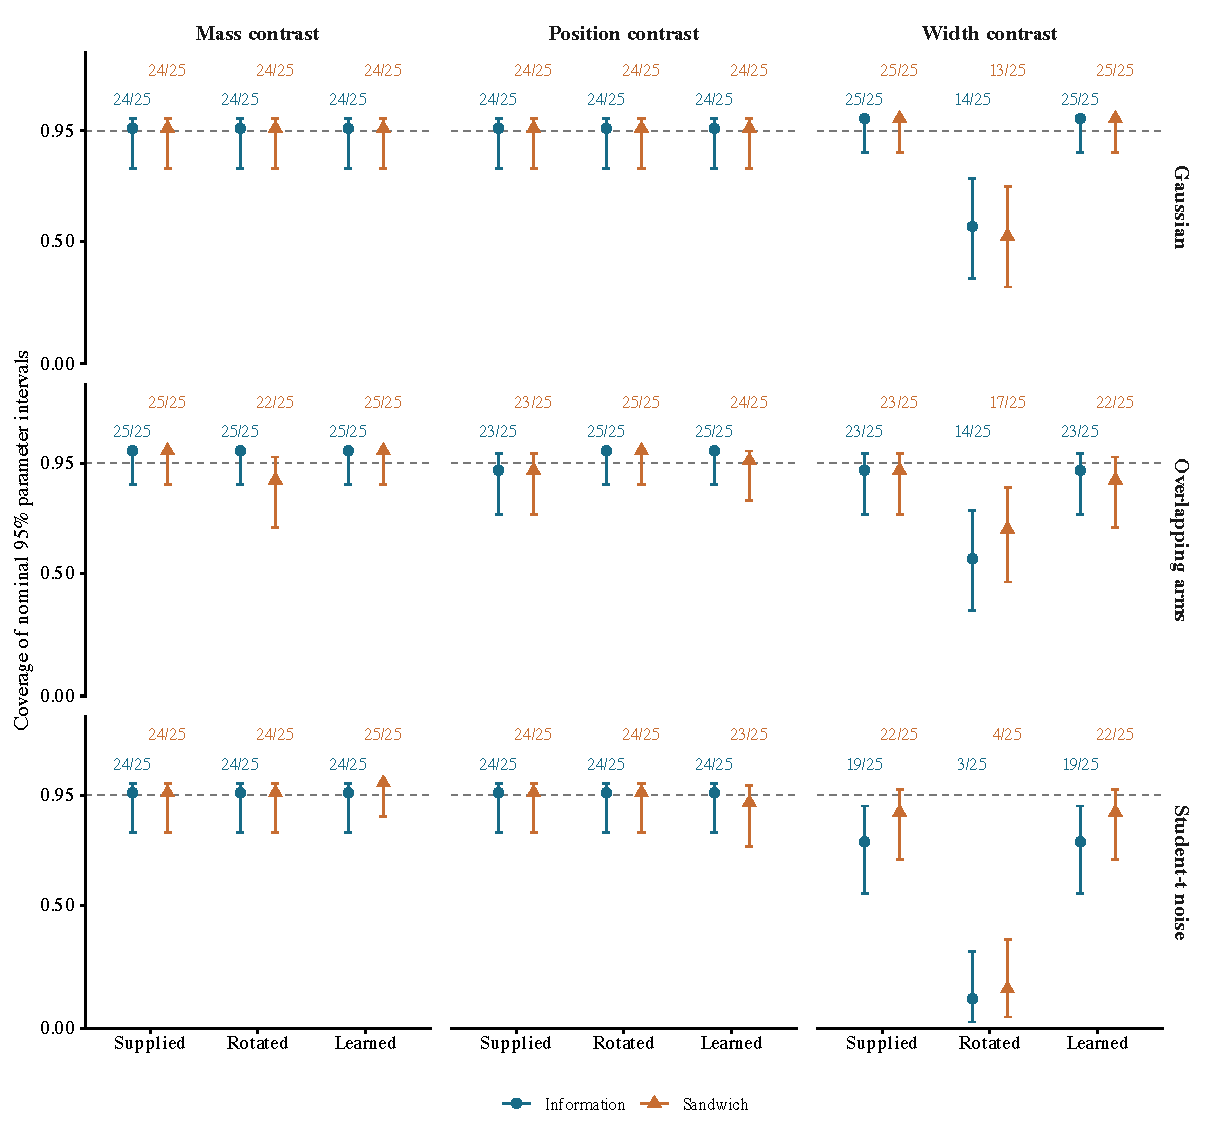
\includegraphics[width=\textwidth,clip]{figures/geometry_interval_coverage.pdf}
\caption{Post-hoc coverage of nominal 95\% parameter intervals for the
geometry/noise study. Columns show the three intended mass, coordinate-mean
and transverse-SD contrasts; rows show Gaussian noise, overlapping arms,
and equal-SD Student-$t_5$ noise. Points and counts use all 25 repetitions.
Bars are exact binomial 95\% Monte Carlo intervals for coverage, not parameter
intervals; the dashed line marks 0.95. Both covariance choices use the same
saved fit and complete six/eight-parameter chart. The 54 displayed cells
follow the prespecified contrast/target pairs; the full numerical record
retains all 378 cells.}
\label{fig:intervals}
\end{figure}

\begin{table}[tbp]
\centering
\footnotesize
\setlength{\tabcolsep}{3pt}
\caption{All intended contrast/target pairs in the saved geometry fits.
Info. and Sand. give covered intervals out of 25 for information and sandwich
covariance. Bias is the mean estimate minus the generating contrast; it is
the same for both covariance choices. SE columns are mean parameter standard
errors, not Monte Carlo SEs. Position is the truncated coordinate mean; SD
is transverse spread. Cross-effects remain in the accompanying complete data.}
\label{tab:geometry-intervals}
\begin{tabular}{@{}lllrrrrr@{}}
\toprule
Condition & Directions & Target & Info. & Sand. & Bias & SE (info.) & SE (sand.) \\
\midrule
Gaussian & Supplied & Mass & 24/25 & 24/25 & 0.00752 & 0.02354 & 0.02354 \\
Gaussian & Supplied & Position & 24/25 & 24/25 & 0.00173 & 0.01186 & 0.01173 \\
Gaussian & Supplied & SD & 25/25 & 25/25 & 0.00153 & 0.00733 & 0.00730 \\
\addlinespace[3pt]
Gaussian & Rotated & Mass & 24/25 & 24/25 & 0.00830 & 0.02389 & 0.02387 \\
Gaussian & Rotated & Position & 24/25 & 24/25 & -0.00048 & 0.01206 & 0.01178 \\
Gaussian & Rotated & SD & 14/25 & 13/25 & -0.01342 & 0.00751 & 0.00716 \\
\addlinespace[3pt]
Gaussian & Learned & Mass & 24/25 & 24/25 & 0.00756 & 0.02354 & 0.02355 \\
Gaussian & Learned & Position & 24/25 & 24/25 & 0.00171 & 0.01186 & 0.01174 \\
Gaussian & Learned & SD & 25/25 & 25/25 & 0.00154 & 0.00738 & 0.00738 \\
\addlinespace[3pt]
Overlap & Supplied & Mass & 25/25 & 25/25 & 0.00697 & 0.02596 & 0.02601 \\
Overlap & Supplied & Position & 23/25 & 23/25 & -0.00149 & 0.01268 & 0.01268 \\
Overlap & Supplied & SD & 23/25 & 23/25 & 0.00305 & 0.00906 & 0.00903 \\
\addlinespace[3pt]
Overlap & Rotated & Mass & 25/25 & 22/25 & 0.01863 & 0.02954 & 0.02859 \\
Overlap & Rotated & Position & 25/25 & 25/25 & 0.00185 & 0.01549 & 0.01505 \\
Overlap & Rotated & SD & 14/25 & 17/25 & -0.01498 & 0.01001 & 0.01069 \\
\addlinespace[3pt]
Overlap & Learned & Mass & 25/25 & 25/25 & 0.00497 & 0.02733 & 0.02744 \\
Overlap & Learned & Position & 25/25 & 24/25 & -0.00135 & 0.01280 & 0.01281 \\
Overlap & Learned & SD & 23/25 & 22/25 & 0.00385 & 0.01191 & 0.01211 \\
\addlinespace[3pt]
Student-$t_5$ & Supplied & Mass & 24/25 & 24/25 & -0.00972 & 0.02373 & 0.02386 \\
Student-$t_5$ & Supplied & Position & 24/25 & 24/25 & 0.00281 & 0.01191 & 0.01183 \\
Student-$t_5$ & Supplied & SD & 19/25 & 22/25 & -0.00655 & 0.00713 & 0.00819 \\
\addlinespace[3pt]
Student-$t_5$ & Rotated & Mass & 24/25 & 24/25 & -0.00688 & 0.02396 & 0.02396 \\
Student-$t_5$ & Rotated & Position & 24/25 & 24/25 & 0.00064 & 0.01203 & 0.01186 \\
Student-$t_5$ & Rotated & SD & 3/25 & 4/25 & -0.02203 & 0.00722 & 0.00760 \\
\addlinespace[3pt]
Student-$t_5$ & Learned & Mass & 24/25 & 25/25 & -0.00979 & 0.02374 & 0.02387 \\
Student-$t_5$ & Learned & Position & 24/25 & 23/25 & 0.00283 & 0.01191 & 0.01183 \\
Student-$t_5$ & Learned & SD & 19/25 & 22/25 & -0.00645 & 0.00718 & 0.00830 \\
\addlinespace[3pt]
\bottomrule
\end{tabular}

\end{table}

\paragraph{Fixed directions in the original mechanism study.}
A separate post-hoc calculation uses all 100 joint fits from the earlier
mechanism study. Its complete six-parameter covariance gives 300 group-target
and 225 contrast-target intervals with no invalid fits. Table~\ref{tab:fixed-intervals}
retains all 21 summary cells. These are different saved fits from those in
the geometry/noise study; their repetitions are not pooled.

\begin{table}[tbp]
\centering
\footnotesize
\setlength{\tabcolsep}{3pt}
\caption{Complete fixed-direction joint-fit interval diagnostic. Covered
counts use 25 repetitions per row. MC intervals are exact binomial 95\%
intervals for coverage; empirical SD and mean SE concern the parameter or
contrast estimator. Contrast rows subtract the independently sampled
reference group. None of these rows describes learned-direction uncertainty.}
\label{tab:fixed-intervals}
\begin{tabular}{@{}lllrrrr@{}}
\toprule
Scope & Group & Target & Covered & 95\% MC interval & Empirical SD & Mean SE \\
\midrule
Group & Reference & Mass & 24/25 & [0.796, 0.999] & 0.01738 & 0.01670 \\
Group & Reference & Position & 24/25 & [0.796, 0.999] & 0.00823 & 0.00870 \\
Group & Reference & Width & 22/25 & [0.688, 0.975] & 0.00369 & 0.00309 \\
\addlinespace[3pt]
Group & Mass & Mass & 22/25 & [0.688, 0.975] & 0.02092 & 0.01673 \\
Group & Mass & Position & 25/25 & [0.863, 1.000] & 0.00486 & 0.00697 \\
Group & Mass & Width & 24/25 & [0.796, 0.999] & 0.00189 & 0.00240 \\
\addlinespace[3pt]
Group & Position & Mass & 24/25 & [0.796, 0.999] & 0.01324 & 0.01637 \\
Group & Position & Position & 24/25 & [0.796, 0.999] & 0.00794 & 0.00810 \\
Group & Position & Width & 25/25 & [0.863, 1.000] & 0.00285 & 0.00298 \\
\addlinespace[3pt]
Group & Width & Mass & 24/25 & [0.796, 0.999] & 0.01758 & 0.01798 \\
Group & Width & Position & 25/25 & [0.863, 1.000] & 0.00972 & 0.00932 \\
Group & Width & Width & 24/25 & [0.796, 0.999] & 0.00713 & 0.00669 \\
\addlinespace[3pt]
Contrast & Mass & Mass & 22/25 & [0.688, 0.975] & 0.02711 & 0.02364 \\
Contrast & Mass & Position & 25/25 & [0.863, 1.000] & 0.00884 & 0.01115 \\
Contrast & Mass & Width & 24/25 & [0.796, 0.999] & 0.00380 & 0.00392 \\
\addlinespace[3pt]
Contrast & Position & Mass & 24/25 & [0.796, 0.999] & 0.02030 & 0.02338 \\
Contrast & Position & Position & 23/25 & [0.740, 0.990] & 0.01095 & 0.01189 \\
Contrast & Position & Width & 23/25 & [0.740, 0.990] & 0.00515 & 0.00430 \\
\addlinespace[3pt]
Contrast & Width & Mass & 24/25 & [0.796, 0.999] & 0.02332 & 0.02454 \\
Contrast & Width & Position & 23/25 & [0.740, 0.990] & 0.01417 & 0.01275 \\
Contrast & Width & Width & 24/25 & [0.796, 0.999] & 0.00826 & 0.00737 \\
\bottomrule
\end{tabular}

\end{table}
\FloatBarrier

\section{All Prespecified Density and Marker Controls}
\label{app:controls}
Every cell below is mean (Monte Carlo SE) over 25 runs. Density scores are
in nats per observation; higher is better. Marker log loss is lower-is-better.
PBMC differences are paired within split, and their SEs describe split
variability in this one collection. No independent-subject uncertainty is
estimated. Simulation score tables retain the same observations per method;
the supplied structural information differs between the SFD ablations and
generic density controls as described in the main text.

\begingroup
\let\paragraph\subsubsection
\subsection{Fixed-geometry density scores}

\begin{tabular}{lrrrr}\toprule
Method & Reference & Mass & Position & Width \\\midrule
Oracle & \numSE{0.146}{0.007} & \numSE{0.232}{0.008} & \numSE{0.144}{0.007} & \numSE{-0.079}{0.008} \\
SFD joint & \numSE{0.143}{0.007} & \numSE{0.229}{0.008} & \numSE{0.142}{0.007} & \numSE{-0.083}{0.008} \\
SFD fixed kernels & \numSE{0.145}{0.007} & \numSE{0.231}{0.008} & \numSE{-0.095}{0.008} & \numSE{-0.179}{0.007} \\
SFD oracle kernels & \numSE{0.145}{0.007} & \numSE{0.231}{0.008} & \numSE{0.143}{0.007} & \numSE{-0.080}{0.008} \\
Gaussian & \numSE{-0.475}{0.007} & \numSE{-0.451}{0.008} & \numSE{-0.601}{0.009} & \numSE{-0.528}{0.009} \\
GMM-4 & \numSE{0.132}{0.007} & \numSE{0.218}{0.008} & \numSE{0.129}{0.007} & \numSE{-0.095}{0.008} \\
GMM-8 & \numSE{0.111}{0.007} & \numSE{0.194}{0.008} & \numSE{0.109}{0.008} & \numSE{-0.117}{0.009} \\
KDE & \numSE{-0.078}{0.009} & \numSE{0.007}{0.008} & \numSE{-0.114}{0.009} & \numSE{-0.240}{0.010} \\
\bottomrule\end{tabular}

\subsection{Geometry/noise density scores}

\paragraph{Gaussian noise.}

\begin{tabular}{lrrrr}\toprule
Method & Reference & Mass & Position & Width \\\midrule
SFD supplied & \numSE{0.123}{0.006} & \numSE{0.226}{0.007} & \numSE{0.142}{0.010} & \numSE{-0.088}{0.007} \\
SFD rotated & \numSE{0.010}{0.005} & \numSE{0.109}{0.008} & \numSE{-0.020}{0.008} & \numSE{-0.152}{0.007} \\
SFD learned angles & \numSE{0.122}{0.006} & \numSE{0.225}{0.007} & \numSE{0.141}{0.010} & \numSE{-0.089}{0.007} \\
Gaussian & \numSE{-0.496}{0.005} & \numSE{-0.454}{0.011} & \numSE{-0.602}{0.008} & \numSE{-0.537}{0.009} \\
GMM-4 & \numSE{0.112}{0.006} & \numSE{0.216}{0.008} & \numSE{0.128}{0.010} & \numSE{-0.101}{0.007} \\
GMM-8 & \numSE{0.088}{0.007} & \numSE{0.193}{0.008} & \numSE{0.105}{0.012} & \numSE{-0.127}{0.008} \\
KDE & \numSE{-0.111}{0.016} & \numSE{-0.001}{0.019} & \numSE{-0.165}{0.020} & \numSE{-0.263}{0.011} \\
\bottomrule\end{tabular}

\paragraph{Overlapping arms.}

\begin{tabular}{lrrrr}\toprule
Method & Reference & Mass & Position & Width \\\midrule
SFD supplied & \numSE{0.199}{0.008} & \numSE{0.289}{0.011} & \numSE{0.166}{0.005} & \numSE{0.067}{0.005} \\
SFD rotated & \numSE{0.139}{0.008} & \numSE{0.212}{0.010} & \numSE{0.045}{0.006} & \numSE{0.043}{0.005} \\
SFD learned angles & \numSE{0.198}{0.008} & \numSE{0.288}{0.011} & \numSE{0.165}{0.005} & \numSE{0.065}{0.005} \\
Gaussian & \numSE{-0.326}{0.011} & \numSE{-0.307}{0.013} & \numSE{-0.401}{0.011} & \numSE{-0.360}{0.008} \\
GMM-4 & \numSE{0.185}{0.009} & \numSE{0.277}{0.011} & \numSE{0.153}{0.006} & \numSE{0.055}{0.005} \\
GMM-8 & \numSE{0.165}{0.008} & \numSE{0.253}{0.011} & \numSE{0.132}{0.006} & \numSE{0.030}{0.006} \\
KDE & \numSE{0.009}{0.013} & \numSE{0.085}{0.017} & \numSE{-0.023}{0.011} & \numSE{-0.074}{0.008} \\
\bottomrule\end{tabular}

\paragraph{Student-t noise.}

\begin{tabular}{lrrrr}\toprule
Method & Reference & Mass & Position & Width \\\midrule
SFD supplied & \numSE{0.157}{0.007} & \numSE{0.264}{0.008} & \numSE{0.173}{0.008} & \numSE{-0.043}{0.007} \\
SFD rotated & \numSE{0.023}{0.006} & \numSE{0.130}{0.008} & \numSE{-0.005}{0.007} & \numSE{-0.121}{0.007} \\
SFD learned angles & \numSE{0.157}{0.007} & \numSE{0.263}{0.008} & \numSE{0.173}{0.008} & \numSE{-0.044}{0.007} \\
Gaussian & \numSE{-0.510}{0.008} & \numSE{-0.450}{0.009} & \numSE{-0.611}{0.007} & \numSE{-0.522}{0.007} \\
GMM-4 & \numSE{0.148}{0.007} & \numSE{0.257}{0.009} & \numSE{0.160}{0.008} & \numSE{-0.052}{0.007} \\
GMM-8 & \numSE{0.129}{0.007} & \numSE{0.236}{0.009} & \numSE{0.138}{0.008} & \numSE{-0.075}{0.007} \\
KDE & \numSE{-0.184}{0.040} & \numSE{-0.035}{0.037} & \numSE{-0.171}{0.026} & \numSE{-0.224}{0.007} \\
\bottomrule\end{tabular}

\subsection{PBMC density and marker controls}

\begin{tabular}{lr}\toprule Method & Test log density \\\midrule

Gaussian & \numSE{-6.422}{0.006} \\

GMM-2 & \numSE{-5.649}{0.011} \\

GMM-4 & \numSE{-5.415}{0.010} \\

GMM-8 & \numSE{-5.367}{0.009} \\

KDE & \numSE{-5.421}{0.009} \\

MST SFD & \numSE{-5.770}{0.018} \\

\bottomrule\end{tabular}

\begin{tabular}{lrr}\toprule Readout & Log loss & Change vs density \\\midrule

PCs & \numSE{0.2526}{0.0036} & \numSE{0.0017}{0.0006} \\

PCs + density & \numSE{0.2509}{0.0033} & \numSE{0.0000}{0.0000} \\

PCs + density + entropy & \numSE{0.2257}{0.0041} & \numSE{-0.0252}{0.0032} \\

PCs + density + SFD & \numSE{0.2029}{0.0056} & \numSE{-0.0481}{0.0044} \\

PCs + density + GMM memberships & \numSE{0.1544}{0.0024} & \numSE{-0.0965}{0.0030} \\

\bottomrule\end{tabular}

\endgroup

\FloatBarrier
\clearpage
\section{External-Family Density Controls}
\label{app:external-density-controls}
These two archived comparisons characterize generic density estimators on
classical and copula distributions. Each uses five repetitions with 1000
training and 1000 independent test observations per scenario. Oracle rows
evaluate the known generating density; neither comparison fits an SFD.
The full score and summary tables accompany the compilation sources.
Finite scores from runs with iteration-limit warnings remain in the means;
the archived status columns identify those runs.

\begin{figure}[H]
\centering
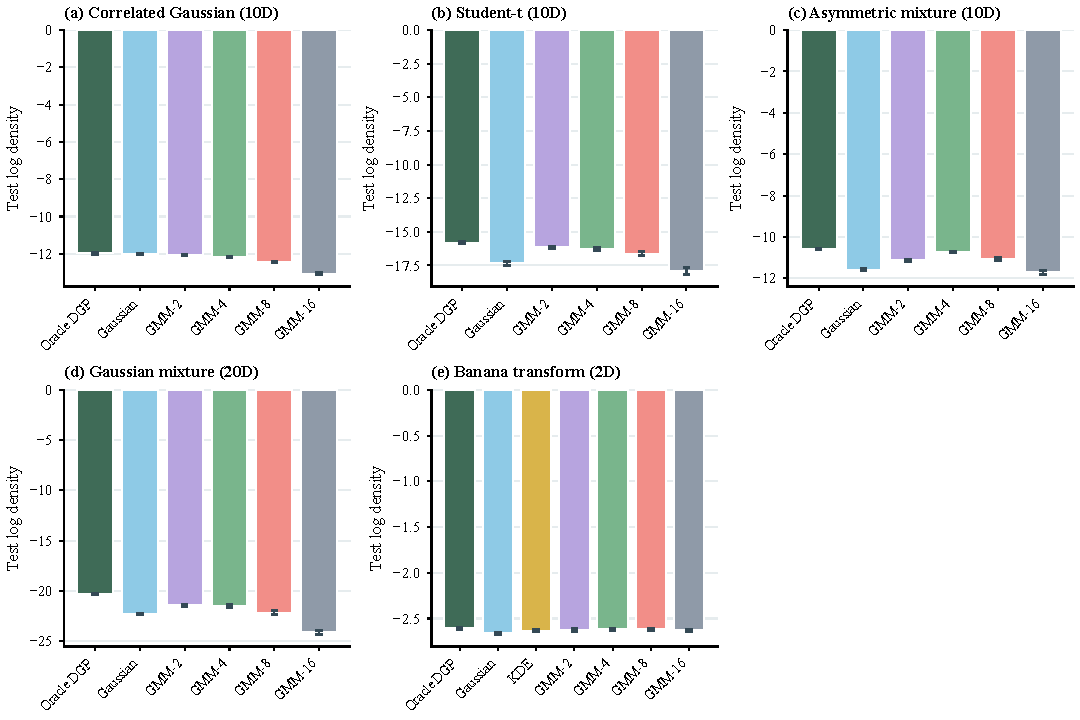
\includegraphics[width=\linewidth,clip]{figures/classical_density_controls.pdf}
\caption{Classical distributions: correlated Gaussian, Student-$t$,
asymmetric Gaussian mixture, Gaussian mixture and banana transform.
Bars show mean test log density and one Monte Carlo SE over five
repetitions. The oracle is the generating density; no SFD is fitted.}
\label{fig:classical-controls}
\end{figure}

\paragraph{Classical-family settings.}
The first three distributions have ten coordinates, the Gaussian mixture
has twenty, and the banana transform has two. GMM sizes are $2,4,8,16$,
with maximum 50 iterations, tolerance $10^{-5}$ and covariance
regularization $10^{-5}$. KDE is included only for the two-dimensional
scenario. The base seed is 20260624. These reduced-scale controls are
separate from the 25-repetition known-skeleton diagnostic.

\clearpage
\paragraph{Copula-family settings.}
The Gaussian and Student-$t$ copulas have ten coordinates; Clayton has five.
The Gaussian correlation is $0.55$. The Student-$t$ copula has correlation
$0.45$ and $4.5$ degrees of freedom. The Clayton parameter is $1.6$.
GMM sizes are $2,4,8,16$, with maximum 60 iterations, tolerance $10^{-5}$
and covariance regularization $10^{-5}$; KDE is included for Clayton only.
The base seed is 20260624. These controls do not include a fitted vine copula.

\begin{figure}[H]
\centering
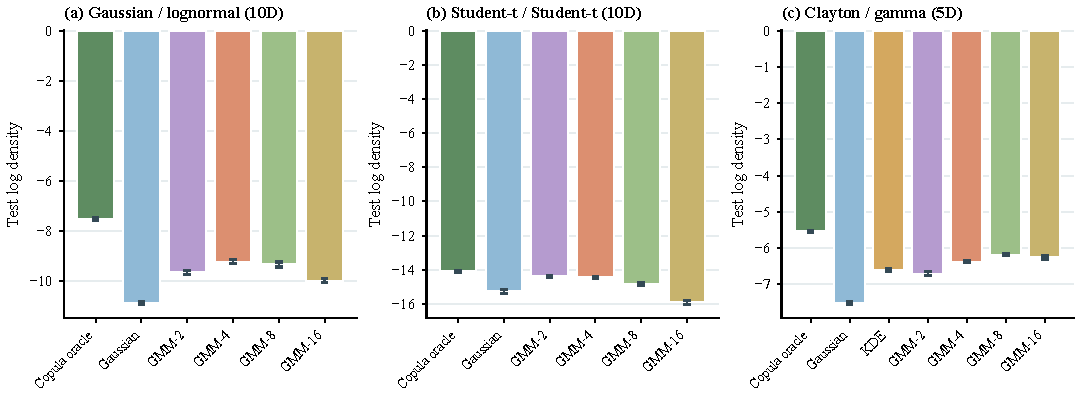
\includegraphics[width=\linewidth,clip]{figures/copula_density_controls.pdf}
\caption{Copula families: Gaussian with lognormal margins, Student-$t$
with Student-$t$ margins, and Clayton with gamma margins. Bars show mean
test log density and one Monte Carlo SE over five repetitions. The oracle
includes the copula and marginal densities; no SFD is fitted.}
\label{fig:copula-controls}
\end{figure}
\FloatBarrier

